% Baccalauréat malgache, série C, 2014 : énoncé.
\TCDBacAttribution{C}{2014}
\providecommand{\dx}{\mathrm{d}x}

%%%%%%%%%%%%%%%%%%%%%%%%%%%%%%%%%%%%%%%%%%%%%%%%%%%%%%%%%%%%%%%%%%%%%%%%%%%%%%%%%%%%%%%%%%%%%%%%%%%%%%%%%%%%%%%%%%%%%%%%%%%%%%%%
\noindent \underline{\textsc{\textbf{Exercice}}} (4 points) \newline
%
      \noindent \underline{\textbf{Partie A}}
            Dans un concours de tir, la cible circulaire se divise en trois zones : A, B et C.
            \begin{figure}[h]
            \centering
            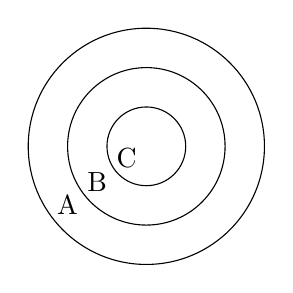
\begin{tikzpicture}[x=.5cm,y=.5cm]
                  \draw(0,0) circle (1);
                  \draw(0,0) circle (2);
                  \draw(0,0) circle (3);
                  \draw (-0.5,-0.3) node[] {$$C$$};
                  \draw (-1.25,-.9) node[] {$$ B $$};
                  \draw (-2.,-1.5) node[] {$$ A $$};
            \end{tikzpicture}
            \end{figure}
            Chaque tire atteint n\'ecessairement l'une des trois zones A, B et C.
            Sachant que $P_C = \frac{1}{6}$ et $P_A$, $P_B$ et $P_C$ forment, dans cet ordre, une progression arithm\'etique.
            \begin{enumerate}
                  \item Calculer $P_A$ et $P_B$.
                  \item On effectue quatre tirs d'une mani\`ere ind\'ependante. Calculer la probabilit\'e d'atteindre au moins une fois la zone C.
                  \item Un joueur tire jusqu'\`a ce que la zone C soit atteinte.
                        Calculer la probabilit\'e de l'\'ev\`enement $E$ : << Le jeu s'arr\^ete au $\text{3}^\text{\`eme}$ tir >>.
                  \item Soit $n\in\mathbb{N}^*$, et $P_n$ la probabilit\'e pour que le jeu s'arr\^ete au $n^\text{i\`eme}$ tir.
                        Ecrire $P_n$ en fonction de $n$.
                        Calculer $\lim_{n\rightarrow+\infty} P_n$.
            \end{enumerate}
      %
      \noindent \underline{\textbf{Partie B}}
            \begin{enumerate}
                  \item Soient $x$ et $y$ deux entiers naturels.
                        D\'emontrer que : $(x+6y)^2 - x^2$ est divisible par 12 et que $(x+6y)^4 - x^4$ est divisible par 24.
                  \item R\'esoudre dans $\mathbb{Z}$ : $3x \equiv 2 \quad [\mathrm{mod}\ 7]$.
                  \item D\'eterminer la base $b$ du syst\`eme de num\'eration dans lequel : $(\bar{12})_{_b} \times (\bar{22})_{_b} = (\bar{314})_{_b}$.
            \end{enumerate}

%%%%%%%%%%%%%%%%%%%%%%%%%%%%%%%%%%%%%%%%%%%%%%%%%%%%%%%%%%%%%%%%%%%%%%%%%%%%%%%%%%%%%%%%%%%%%%%%%%%%%%%%%%%%%%%%%%%%%%%%%%%%%%%%
\noindent \underline{\textsc{\textbf{PROBLEME I}}} (7 points) \newline
%
      \textbf{Les parties I et II sont ind\'ependantes.} 
      
      On consid\`ere un triangle quelconque $AOB$,
      $AOE$ est un triangle direct isoc\`ele et rectangle en $E$,
      $BAC$ est un triangle direct isoc\`ele et rectangle en $C$,
      $OBD$ est un triangle direct isoc\`ele et rectangle en $D$.
      \begin{figure}[h!]
      \centering
            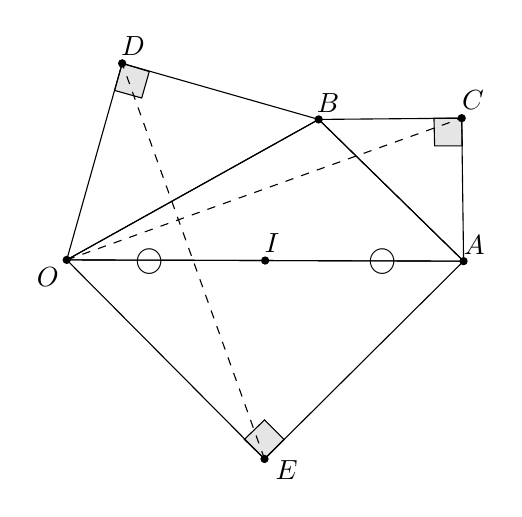
\begin{tikzpicture}[x=.8cm,y=.8cm]
                  \draw[fill=black,fill opacity=0.1] (2.52,0.09) -- (2.53,-0.35) -- (2.97,-0.35) -- (2.96,0.09) -- cycle; 
                  \draw[fill=black,fill opacity=0.1] (-2.55,0.53) -- (-2.12,0.41) -- (-2,0.83) -- (-2.43,0.96) -- cycle; 
                  \draw[fill=black,fill opacity=0.1] (0.14,-5.01) -- (-0.17,-4.7) -- (-0.49,-5.01) -- (-0.17,-5.32) -- cycle; 
                  \draw (2.99,-2.18)-- (0.69,0.07);
                  \draw (0.69,0.07)-- (-3.31,-2.16);
                  \draw (-3.31,-2.16)-- (2.99,-2.18);
                  \draw (-3.31,-2.16)-- (-0.17,-5.32);
                  \draw (-0.17,-5.32)-- (2.99,-2.18);
                  \draw (2.99,-2.18)-- (-3.31,-2.16);
                  \draw (-2.43,0.96)-- (-3.31,-2.16);
                  \draw (-3.31,-2.16)-- (0.69,0.07);
                  \draw (0.69,0.07)-- (-2.43,0.96);
                  \draw (0.69,0.07)-- (2.96,0.09);
                  \draw (2.96,0.09)-- (2.99,-2.18);
                  \draw (2.99,-2.18)-- (0.69,0.07);
                  \draw [dash pattern=on 3pt off 3pt] (-3.31,-2.16)-- (2.96,0.09);
                  \draw [dash pattern=on 3pt off 3pt] (-0.17,-5.32)-- (-2.43,0.96);
                  \fill [color=black] (2.99,-2.18) circle (1.5pt);
                  \draw[color=black] (3.16,-1.92) node {$A$};
                  \fill [color=black] (0.69,0.07) circle (1.5pt);
                  \draw[color=black] (0.84,0.33) node {$B$};
                  \fill [color=black] (-3.31,-2.16) circle (1.5pt);
                  \draw[color=black] (-3.61,-2.44) node {$O$};
                  \fill [color=black] (-0.17,-5.32) circle (1.5pt);
                  \draw[color=black] (0.18,-5.5) node {$E$};
                  \fill [color=black] (2.96,0.09) circle (1.5pt);
                  \draw[color=black] (3.14,0.37) node {$C$};
                  \fill [color=black] (-2.43,0.96) circle (1.5pt);
                  \draw[color=black] (-2.26,1.23) node {$D$};
                  \fill [color=black] (-0.16,-2.17) circle (1.5pt);
                  \draw[color=black] (-0.05,-1.9) node {$I$};
                  %%%%
                  \draw (-2 , -3.5) node {$\diagup\!\!\!\diagup$};
                  \draw (1.7 , -3.5) node {$\diagdown\!\!\!\diagdown$};
                  %
                  \draw (-2 , -2.18) node {$\bigcirc$};
                  \draw (1.7 , -2.18) node {$\bigcirc$};
                  %
                  \draw (-1 , .55) node {$\diagup\!\!\!\diagup\!\!\!\diagup$};
                  \draw (-2.75 , -.25) node {\rotatebox{40}{$\diagdown\!\!\!\diagdown\!\!\!\diagdown$}};
                  %
                  \draw (3 , -.95) node {$\diagup$};
                  \draw (1.75 , .1) node {$\diagup$};
            \end{tikzpicture}
      \end{figure}
      On se propose de d\'emontrer que les droites $(OC)$ et $(ED)$ sont perpendiculaires et que $OC = ED$.
      %
      
      %
      \noindent \underline{\textbf{PARTIE I :}} \underline{M\'ethode 1 :} Utilisation des transformations.      \\
            On note :
                  \begin{itemize}
                        \item $S_1$ la similitude plane directe de centre $A$ qui transforme $C$ en $B$,
                        \item $S_2$ la similitude plane directe de centre $O$ qui transforme $B$ en $D$,
                        \item $f = S_2 \circ S_1$.
                  \end{itemize}
            %
            \begin{enumerate}
                  \item \begin{enumerate}
                              \item D\'eterminer le rapport et l'angle de chacun des transformations $S_1$ et $S_2$.
                              \item Prouver que $f$ est une rotation dont on pr\'ecisera l'angle.
                        \end{enumerate}
                  \item D\'eterminer l'image de $I$ par $S_1$ et celle de $E$ par $S_2$.
                        En d\'eduire que $I$ est invariant par $f$.
                  \item On appelle $R$ la rotation de centre $I$ et d'angle $\theta = \frac{\pi}{2}$.
                        \begin{enumerate}
                              \item D\'eterminer $R(O)$ et $R(C)$.
                              \item En d\'eduire que $(OC)$ et $(ED)$ sont perpendiculaires et que $OC = ED$.
                        \end{enumerate}
            \end{enumerate}
      %
      
      %
      \noindent \underline{\textbf{PARTIE II :}} \underline{M\'ethode 2 :} Utilisation des nombres complexes.
            Le plan complexe est rapport\'e \`a un rep\`ere orthonorm\'e direct $(O ; \vec{u} , \vec{v} )$ avec $\vec{u} = \overrightarrow{OI}$.
            On note $b$ l'affixe de $B$.
            \begin{enumerate}
                  \item Calculer en fonction de $b$ l'affixe de $C$ et l'affixe de $D$.
                  \item Calculer l'affixe $Z_E$ de $E$.
                  \item \begin{enumerate}
                              \item D\'emontrer que $\displaystyle{\frac{Z_D - Z_E}{Z_C - Z_O} = i}$.
                              \item En d\'eduire que $(OC)$ et $(ED)$ sont perpendiculaires et que $OC = ED$.
                        \end{enumerate}
            \end{enumerate}
%
%%%%%%%%%%%%%%%%%%%%%%%%%%%%%%%%%%%%%%%%%%%%%%%%%%%%%%%%%%%%%%%%%%%%%%%%%%%%%%%%%%%%%%%%%%%%%%%%%%%%%%%%%%%%%%%%%%%%%%%%%%%%%%%%
\noindent \underline{\textsc{\textbf{PROBLEME II}}} (9 points) \newline
      On consid\`ere la fonction num\'erique $f$ d\'efinie sur $\mathbb{R}$ par :
      \[
      f(x) = \begin{multiform}
                   (1-x) \; \expo{x}  \text{ si }  x < 1 \\
                   x - 1 + \ln \frac{2x}{x+1}  \text{ si }  x \geq 1.
             \end{multiform}
      \]
      On d\'esigne par $(C)$ sa courbe repr\'esentative dans un plan muni d'un 
      rep\`ere orthonorm\'e $(O ; \vec{\imath} , \vec{\jmath})$ d'unit\'e 1~cm.
     %
     
     %
      \noindent \underline{\textbf{PARTIE I :}}
            \begin{enumerate}
                  \item Prouver que $f$ est continue en $x_0 = 1$.
                  \item \begin{enumerate}
                              \item V\'erifier que pour tout $x > 1$ :
                                    $$
                                    \frac{f(x)-f(1)}{x-1} = 1 + \frac{\ln x}{x-1} - \frac{\ln (x+1) - \ln 2}{x-1}
                                    .$$
                                    D\'emontrer que $f$ est d\'erivable \`a droite en $1$ et que $f'_d (1) = \frac{3}{2}$.
                              \item Etudier la d\'erivabilit\'e \`a gauche de $f$ en $x_0 = 1$.
                        \end{enumerate}
                  \item Calculer $\displaystyle{\lim_{x\rightarrow-\infty} f(x)}$ et $\displaystyle{\lim_{x\rightarrow+\infty} f(x)}$.
                  \item \begin{enumerate}
                              \item Etudier le sens de variation de $f$ sur son domaine de d\'efinition.
                              \item Dresser le tableau de variation de $f$.
                        \end{enumerate}
                  \item On pose $\varphi(x) = f(x)-x+1-\ln 2$.
                        Calculer $\displaystyle{\lim_{x\rightarrow+\infty}\varphi(x)}$.
                        Que signifie ce r\'esultat pour la courbe $(C)$\,?
                  \item Tracer les demi-tangentes au point d'abscisse $x_0 = 1$, l'asymptote et la courbe $(C)$.
            \end{enumerate}
     %
     
     %
      \noindent \underline{\textbf{PARTIE II :}}
            \begin{enumerate}
                  \item On consid\`ere l'\'equation diff\'erentielle 
                        $(E) : y' - y = (-2x+1) \; \expo{x}$.
                        Soit $g$ une solution de $(E)$, d\'emontrer que toute fonction $\varphi$ d\'efinie par $\varphi(x) = \expo{-x} g(x)$ 
                        v\'erifie $\varphi'(x) = -2x+1$.
                        En d\'eduire la solution de $(E)$ qui prend la valeur $1$ en $x_0 = 0$.
                  \item R\'esoudre dans $[0 ; 2\pi]$ l'\'equation 
                        $\sqrt{3} \cos x + \sin x - \sqrt{2} = 0$.
                  \item Soit la suite num\'erique $(I_n)_{n\in\mathbb{N}^*}$ d\'efinie par :
                        \[
                              I_n = \frac{1}{n!} \int_{0}^{1} (1-x)^n \expo{x} \dx.
                        \]
                        \begin{enumerate}
                              \item Calculer $I_1$.
                                    Interpr\'eter g\'eom\'etriquement ce r\'esultat.
                              \item Trouver une relation de r\'ecurrence entre $I_{n+1}$ et $I_n$.
                                    En d\'eduire que pour tout $n\in\mathbb{N}^*$ : $I_n = e - 1 - \sum_{k=1}^{n} \frac{1}{k!}$.
                              \item D\'emontrer que pour tout $n\in\mathbb{N}^*$ : 
                                    $\displaystyle{
                                    \frac{1}{(n+1)!} \leq I_n \leq \frac{e}{(n+1)!}
                                    }.$
                                    En d\'eduire 
                                    $\displaystyle{
                                    \lim_{n\rightarrow+\infty} \left( \sum_{k=1}^{n} \frac{1}{k!} \right)
                                    }.$
                        \end{enumerate}
                  On donne : $\expo{-3} \simeq 0,05$ ; $\expo{-2} \simeq 0,14$ ; $\expo{-1} \simeq 0,37$ ; $\ln 2 \simeq 0,7$ et $\ln 3 \simeq 1,1$.
            \end{enumerate}
      
%%%%%%%%%%%%%%%%%%%%%%%%%%%%%%%%%%%%%%%%%%%%%%%%%%%%%%%%%%%%%%%%%%%%%%%%%%%%%%%%%%%%%%%%%%%%%%%%%%%%%%%%%%%%%%%%%%%%%%%%%%%%%%%%





































